\chapter{Design and Implementation of the FiberGate AI Service}

\section*{Introduction}
\addcontentsline{toc}{section}{Introduction}

This chapter documents the engineering trajectory of the FiberGate AI Service, the second pillar of the FiberGate ecosystem. It covers the model-selection study leading to the adoption of LayoutLMv3, the construction of an 872-document annotated corpus, the design and training of two task-specific heads for classification and field extraction, the BIO sequence-labelling strategy driving per-token supervision, the experimental evaluation on the held-out test set, and the lifecycle framework ensuring continuous improvement in production.

\section{Technology Evaluation and Proof-of-Concept Findings}

The deployed system constitutes the second iteration of the FiberGate AI Service. Its design was shaped by a first prototype evaluated under near-production conditions, whose limitations and the resulting model-selection study are reviewed below.

\subsection{First-Generation Hybrid Pipeline: Design and Limitations}

The first prototype used a different processing branch for each document type. It combined simple rule-based extraction with a small language model running on a local machine. The three branches ran in parallel and were served through a FastAPI back-end with an asynchronous job queue:

-- 	Digital information sheets (text-based PDFs) were handled by pdfplumber and regular expressions.

-- 	Scanned authorisation permits and mandates were processed by Tesseract 5 (with a French model), regular expressions, and a local Ollama deployment of the qwen2.5:1.5b model.

-- 	The three remaining document types went through Tesseract and Ollama for classification only.

Testing this prototype revealed three main problems. Each one led to a specific decision in the second version:

-- 	\textbf{Regular expressions were fragile.} The pattern used to read the permit reference number had to be rewritten three times during testing, because the format of the documents kept changing. This level of manual work cannot scale to the number of templates seen in production.

-- 	\textbf{The small language model was not reliable enough.} The qwen2.5:1.5b model returned invalid JSON in about one mandate call out of six. More importantly, it had no understanding of document layout, so it could not tell apart a target field value from the same text appearing elsewhere on the page. A text-only model was clearly not enough.

-- 	\textbf{Per-type branching was costly to maintain.} Every new document type needed its own regular expressions and its own prompts, with nothing shared between branches. The work grew linearly with the number of supported types.

Two parts of the first prototype worked well and were reused without changes: the Tesseract OCR step and the rule-based engine that turns extracted values into a LOC PAR completeness verdict. Both are deterministic and contain no learned parameters, which made them easy to keep.

\begin{figure}[H]
  \centering
  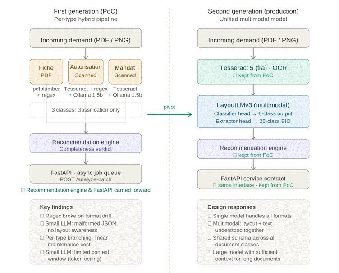
\includegraphics[width=0.85\textwidth,max width=\textwidth]{images/image56.png}
  \caption{\textit{\textbf{Figure 5.1.} Architectural comparison between the first-generation (proof-of-concept) and the second-generation unified multimodal pipeline.}}
  \label{fig:image56}
\end{figure}

\subsection{Multimodal Model Comparative Analysis and Selection of LayoutLMv3}

The first version made one thing clear: we needed a model that could read text, page layout, and the image of the page together, inside one single architecture. Text-only classifiers miss visual signals such as stamps, table borders, and header shapes that carry a lot of meaning in administrative documents. Image-only classifiers, on the other hand, miss the text that actually contains most of the information we want. A multimodal model was therefore necessary.

Six open-source document AI models were studied. Each was compared on five criteria: the modalities it can read, its number of parameters, its peak GPU memory, its licence, and how well it fits the project constraints. The results are gathered in Table 5.1.

\begin{table}[H]
  \centering
  \caption{\textit{\textbf{Table 5.1.} Comparison of open-source document AI models evaluated for the FiberGate AI Service.}}
  \renewcommand{\arraystretch}{1.3}
  \footnotesize
  \begin{tabularx}{\textwidth}{|X|X|X|X|X|X|X|}
    \hline
    \textbf{Model} & \textbf{Modalities} & \textbf{Image Method} & \textbf{Params} & \textbf{VRAM} & \textbf{Licence} & \textbf{Decision} \\ \hline
    LayoutLMv1 (Microsoft, 2020) & Text + layout & None & 160 M & 6 GB & MIT & \textbf{Rejected:} no image input. \\ \hline
    LayoutLMv2 (Microsoft, 2021) & Text, layout, image & Faster R-CNN (CNN) & 426 M & 18 GB & MIT & \textbf{Rejected:} heavy detector pushes memory above a single GPU. \\ \hline
    \textbf{LayoutLMv3 [Selected]} (Microsoft, 2022) & Text, layout, image & 14 $\times$ 14 image patches & 125 M & 7 GB & CC BY-NC & \textbf{Selected:} unified design, smallest multimodal model, fits one GPU. \\ \hline
    LiLT (HuggingFace, 2022) & Text + layout & None & 250 M & 7 GB & MIT & \textbf{Rejected:} no image input. \\ \hline
    Donut (NAVER, 2022) & Image only & Swin + seq2seq & 200 M & 5 GB & MIT & \textbf{Rejected:} slow decoder, often hallucinates text. \\ \hline
    UDOP (Microsoft, 2023) & Text, layout, image & ViT + T5 & 742 M & 24 GB & MIT & \textbf{Rejected:} 6$\times$ larger than LayoutLMv3 and exceeds GPU memory. \\ \hline
  \end{tabularx}
\end{table}

LayoutLMv3 was selected directly from this study. Its main idea is a unified self-attention block that reads text tokens, layout coordinates, and image patches together, instead of using a separate encoder for each modality. With 125 M parameters and 7 GB of VRAM, it fits well on a single consumer GPU. Its pre-training corpus (IIT-CDIP) is mainly in English, so adaptation to the French administrative style is done through fine-tuning on the project corpus described in the next section.

\section{Dataset Construction and Preparation}

\subsection{Data Collection, Annotation Methodology, and Schema Definition}

The corpus is made of scanned administrative documents coming from French urban-planning offices. They were collected in three batches through the Agilis platform. In total, 1,008 unique documents were gathered. Out of these, 872 (86.5\%) were kept for annotation. The remaining 136 documents were removed because their OCR quality was too low (heavy stamps, low contrast, low resolution) or because they were exact duplicates of documents already in the corpus. The numbers per batch are reported in Table 5.2.

\begin{table}[H]
  \centering
  \caption{\textit{\textbf{Table 5.2.} Document collection batches and annotation coverage.}}
  \renewcommand{\arraystretch}{1.3}
  \footnotesize
  \begin{tabularx}{\textwidth}{|>{\raggedright\arraybackslash}p{2.3cm}|X|X|X|}
    \hline
    \textbf{Batch} & \textbf{Documents} & \textbf{Annotated} & \textbf{Source} \\ \hline
    Batch 1 & 420 & 368 (87.6\%) & Agilis, urban-planning offices \\ \hline
    Batch 2 & 358 & 308 (86.0\%) & Agilis, urban-planning offices \\ \hline
    Batch 3 & 230 & 196 (85.2\%) & Agilis, urban-planning offices \\ \hline
    Total & 1,008 & 872 (86.5\%) &  \\ \hline
  \end{tabularx}
\end{table}

Annotation was done with Label Studio. To follow the GDPR rules discussed in Chapter 4, a local Python HTTP server with CORS headers was set up to send the document images to the Label Studio interface. This way, all sensitive data stayed on the local machine and was never sent to an external service. Each document received two kinds of label: one document-level class chosen from six categories, and zero or more field-level bounding boxes drawn from a twelve-class schema.

We chose bounding boxes instead of free-text labels for two reasons. First, LayoutLMv3 already understands layout signals, so bounding boxes give the model exactly the kind of input it expects. Second, a bounding box keeps the spatial difference between, for example, a project address printed in the body of a document and the same address printed in the letterhead. With free-text labels, this difference would be lost exactly where it matters most. The six document classes follow the LOC PAR validation checklist already used by the team, so the labels match the vocabulary that consultants know. Table 5.3 lists each class with its extractable fields.

\begin{table}[H]
  \centering
  \caption{\textit{\textbf{Table 5.3.} Document classes and associated extractable field classes.}}
  \renewcommand{\arraystretch}{1.3}
  \begin{tabularx}{\textwidth}{|X|X|}
    \hline
    \textbf{Document Class} & \textbf{Field Classes} \\ \hline
    Information Sheet & Urbanisme permit number, DLPI, Commercial operator, Total number of housings, Total number of residential housings, Total number of professional housings, Total number of Lot/Macrolot, Street address, Mandate disposition \\ \hline
    Urbanisme Permit & Urbanisme permit number \\ \hline
    Mandate & Representative information: Full name, Phone number, Email \\ \hline
    Addressing Certificate & Street address \\ \hline
    Mass Plan & Classification only \\ \hline
    Situation Plan & Classification only \\ \hline
  \end{tabularx}
\end{table}

\begin{figure}[H]
  \centering
  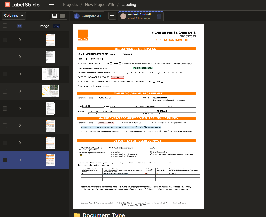
\includegraphics[width=0.85\textwidth,max width=\textwidth]{images/image57.png}
  \caption{\textit{\textbf{Figure 5.3.} Label Studio annotation interface}}
  \label{fig:image57}
\end{figure}

\subsection{Dataset Statistical Analysis and Class Imbalance Mitigation}

The 872 annotated documents were divided into training, validation, and test sets using a 70/15/15 ratio. The split was applied at the source-PDF level, not at the page level. This choice is very important. Many documents contain several pages, and pages from the same folder share OCR templates, layouts, and often the same field values. If the split were done at the page level, pages from the same folder could appear in both the training set and the test set, which would cause data leakage and make the scores look better than they really are. A split at the source-PDF level avoids this problem by construction. The aggregate statistics of the dataset are reported in Table 5.4.

\begin{figure}[H]
  \centering
  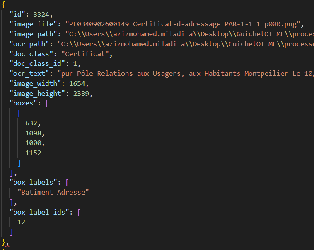
\includegraphics[width=0.85\textwidth,max width=\textwidth]{images/image59.png}
  \caption{\textit{\textbf{Figure 5.4.} Training data sample showing the structured JSON representation of an annotated document, including OCR tokens, normalised bounding boxes, and the assigned class and field labels.}}
  \label{fig:image59}
\end{figure}

\begin{table}[H]
  \centering
  \caption{\textit{\textbf{Table 5.4.} Aggregate dataset statistics across all annotated documents.}}
  \renewcommand{\arraystretch}{1.3}
  \begin{tabularx}{\textwidth}{|X|X|}
    \hline
    \textbf{Metric} & \textbf{Value} \\ \hline
    Total annotated documents & 872 \\ \hline
    Training samples (70\%) & 609 \\ \hline
    Validation samples (15\%) & 130 \\ \hline
    Test samples (15\%) & 133 \\ \hline
    Average words per document & 348 \\ \hline
    Maximum words in a single document & 10,039 \\ \hline
    Documents exceeding 512 tokens & 88 / 872 (10.1\%) \\ \hline
    Average image resolution & 1,655 $\times$ 2,335 pixels \\ \hline
    Class imbalance ratio (max/min) & 8.1$\times$ (Authorisation / Mandate) \\ \hline
    Training documents with bounding-box annotations & 335 / 609 (55\%) \\ \hline
    Average bounding boxes per annotated document & 3.1 \\ \hline
  \end{tabularx}
\end{table}

The class distribution is very unbalanced. The Authorisation Permit class represents 31.8\% of the corpus (277 documents), while the Mandate class represents only 3.9\% (34 documents). This gives a maximum-to-minimum ratio of 8.1. This imbalance must be handled during training and kept in mind when reading macro-averaged scores. The full per-class composition is given in Table 5.5.

\begin{table}[H]
  \centering
  \caption{\textit{\textbf{Table 5.5.} Document classes with sample counts, proportions, and extracted fields.}}
  \renewcommand{\arraystretch}{1.3}
  \footnotesize
  \begin{tabularx}{\textwidth}{|X|X|X|X|}
    \hline
    \textbf{Class} & \textbf{Total} & \textbf{\% Dataset} & \textbf{Extracted Fields} \\ \hline
    Authorisation Permit & 277 & 31.8\% & Urbanisme permit number \\ \hline
    Situation Plan & 168 & 19.3\% & Classification only \\ \hline
    Information Sheet & 151 & 17.3\% & Permit number, DLPI, Commercial operator, Total / residential / professional housings, Lot/Macrolot, Street address, Mandate disposition \\ \hline
    Mass Plan & 139 & 15.9\% & Classification only \\ \hline
    Certificate & 103 & 11.8\% & Street address \\ \hline
    Mandate & 34 & 3.9\% & Full name, Phone number, Email \\ \hline
  \end{tabularx}
\end{table}

\begin{figure}[H]
  \centering
  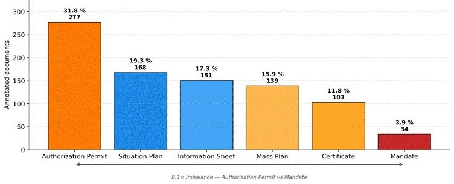
\includegraphics[width=0.85\textwidth,max width=\textwidth]{images/image60.png}
  \caption{\textit{\textbf{Figure 5.5.} Annotated dataset distribution: per-class document counts illustrating the 8.1$\times$ class-imbalance ratio between Authorisation Permit and Mandate.}}
  \label{fig:image60}
\end{figure}

To deal with this imbalance during training, each class received a weight inversely proportional to its frequency in the training set, computed as:

wi = N / (k $\cdot$ ni)

where \textit{N} denotes the total number of training documents (872), \textit{k} the number of classes (6), and \textit{ni} the number of training samples in class \textit{i}.

The weights were then normalised so that they sum to k, and were passed to the CrossEntropyLoss function. The effect is simple: rare classes contribute a larger gradient during training, which prevents the model from focusing too much on the most frequent classes. The resulting per-class weights are reported in Table 5.6.

\begin{table}[H]
  \centering
  \caption{\textit{\textbf{Table 5.6.} Inverse-frequency class weights applied to CrossEntropyLoss during classifier training.}}
  \renewcommand{\arraystretch}{1.3}
  \footnotesize
  \begin{tabularx}{\textwidth}{|X|X|X|X|}
    \hline
    \textbf{Class} & \textbf{Train N} & \textbf{Weight} & \textbf{Effect on Training} \\ \hline
    Authorisation Permit & 192 & 0.304 & Penalised, most frequent class \\ \hline
    Situation Plan & 123 & 0.466 & Slightly penalised \\ \hline
    Mass Plan & 99 & 0.543 & Slightly penalised \\ \hline
    Information Sheet & 108 & 0.612 & Near-neutral \\ \hline
    Certificate & 68 & 0.786 & Slightly boosted \\ \hline
    Mandate & 19 & 3.290 & Strongly boosted, rarest class \\ \hline
  \end{tabularx}
\end{table}

\section{Model Architecture and Implementation}

With the dataset characterised, attention turns to the model design. This section first details the LayoutLMv3 backbone, then describes the two task-specific heads attached to it, before specifying the preprocessing pipeline that converts a raw scanned document into the input format expected by the model.

\subsection{LayoutLMv3: Unified Multimodal Transformer Architecture}

LayoutLMv3 reads three input streams inside a single transformer encoder. The text stream comes from applying a WordPiece subword tokeniser to the Tesseract OCR output. The layout stream is made of normalised bounding boxes in the range [0, 1000], one per text token. The image stream is built by resizing the page to 224 $\times$ 224 pixels, cutting it into a 14 $\times$ 14 grid of patches, and projecting each patch into a 768-dimensional vector through a linear layer.

The three streams are then projected into a shared 768-dimensional embedding space and passed through twelve transformer encoder layers with multi-head self-attention (12 attention heads; 86 M parameters in the backbone). A special [CLS] token is added at the start of every input sequence. Its final hidden state is used as a compact representation of the whole document, which the classification head then reads. The architecture is shown in Figure 5.6.

\begin{figure}[H]
  \centering
  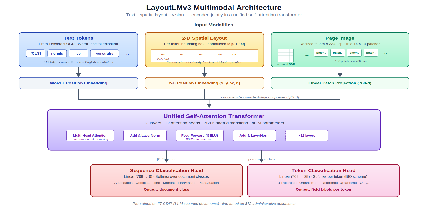
\includegraphics[width=0.85\textwidth,max width=\textwidth]{images/image61.png}
  \caption{\textit{\textbf{Figure 5.6.} LayoutLMv3 multimodal architecture: text tokens, two-dimensional spatial layout, and page-image patches are encoded jointly in a unified self-attention transformer.}}
  \label{fig:image61}
\end{figure}

The microsoft/layoutlmv3-base checkpoint was pre-trained on IIT-CDIP, a large English-language collection of scanned business documents, using three self-supervised objectives:

-- 	\textbf{Masked Language Modelling (MLM):} 15\% of the text tokens are masked and the model has to reconstruct them from the surrounding context, like in the original BERT.

-- 	\textbf{Masked Image Modelling (MIM):} 40\% of the image patches are masked and the model has to predict a discrete visual token for each one, following the BEiT framework.

-- 	\textbf{Word-Patch Alignment (WPA):} a binary task in which the model has to decide whether a text token and an image patch are at the same place on the page. This encourages the model to learn how text and image relate to each other.

Together, these three objectives produce a backbone that already understands text, visual structure, and the link between the two. The fine-tuning steps in Section 5.4 build on this backbone and adapt it to the French administrative style by training on the project corpus .

\subsection{Task-Specific Head Design: Document Classifier and Field Extractor}

Two task-specific heads are attached to the shared LayoutLMv3 backbone. Because both heads use the same backbone, document classification and field extraction are done in a single forward pass at inference time, which saves both time and memory.

-- 	\textbf{Document classification head.} A linear layer that maps the 768-dimensional final hidden state of the [CLS] token to six logits, one per document class. A softmax then turns these logits into a probability distribution. The class with the highest probability is the prediction, and that probability is the confidence score used by the gating policy described in Section 5.5.3.

\textbf{Field extraction head.} A linear layer that maps the 768-dimensional hidden state of each token to twenty-five logits, following a BIO scheme. BIO stands for Beginning, Inside, and Outside. Each token receives either B-\{field\} if it is the first token of a span, I-\{field\} if it continues such a span, or O if it is outside any span. With twelve field types and one shared O class, the label space contains 1 + 12 $\times$ 2 = 25 categories per token .

\section{Model Training Methodology}

Training is done in two phases. The classifier is fine-tuned first, starting from microsoft/layoutlmv3-base. Its trained backbone weights are then used to initialise the extractor, whose head is the only part trained from scratch.

\subsection{Document Classifier Training Procedure}

The classifier is trained with the AdamW optimiser at a learning rate of 2 $\times$ 10\textsuperscript{$-$}\textsuperscript{5}. A linear warm-up over the first 10\% of training steps is followed by a linear decay to zero. A weight decay of 0.01 provides mild L2 regularisation. The effective batch size is 16, obtained by combining a per-step batch size of 4 with 4 gradient-accumulation steps. This balance keeps the gradient stable while staying within the memory budget of a single consumer GPU. The schedule allows up to twenty epochs, with early stopping on the validation loss (patience 5). FP16 mixed precision is enabled when CUDA is available, which cuts the GPU memory footprint in half without harming convergence. The class-imbalance correction from Section 5.2.2 is applied through inverse-frequency weights inside the CrossEntropyLoss term. Table 5.7 reports the full configuration.

\begin{table}[H]
  \centering
  \caption{\textit{\textbf{Table 5.7.} Document classifier training configuration.}}
  \renewcommand{\arraystretch}{1.3}
  \begin{tabularx}{\textwidth}{|X|X|X|}
    \hline
    \textbf{Hyperparameter} & \textbf{Value} & \textbf{Rationale} \\ \hline
    Base checkpoint & microsoft/layoutlmv3-base & Pre-trained on 11 M document pages \\ \hline
    Learning rate & 2 $\times$ 10\textsuperscript{$-$}\textsuperscript{5} & Standard value for transformer fine-tuning \\ \hline
    Effective batch size & 16 (4 $\times$ 4 grad. accum.) & Good balance between memory and stability \\ \hline
    Training epochs & 20 (early stopping, patience 5) & Stops when validation loss stops improving \\ \hline
    Optimiser / weight decay & AdamW / 0.01 & Mild L2 regularisation \\ \hline
    LR schedule & Warm-up 10\%, then linear decay & Avoids early-epoch oscillation \\ \hline
    Mixed precision & FP16 when CUDA available & Cuts GPU memory in half \\ \hline
    Class weights & Inverse-frequency (Table 5.6) & Corrects 8.1$\times$ imbalance \\ \hline
    Max sequence / image & 512 tokens / 224 $\times$ 224 px & LayoutLMv3 input limits \\ \hline
    Base checkpoint & microsoft/layoutlmv3-base & Pre-trained on 11 M document pages \\ \hline
    Learning rate & 2 $\times$ 10\textsuperscript{$-$}\textsuperscript{5} & Standard value for transformer fine-tuning \\ \hline
  \end{tabularx}
\end{table}

\subsection{BIO Sequence Labelling Strategy for Field Extraction}

Turning Label Studio bounding-box annotations into per-token training targets is the most delicate preprocessing step in the whole pipeline. It transforms a sparse ground truth (one rectangle per field per page) into a dense sequence of BIO class indices aligned with the tokenised text, which the cross-entropy loss can use during back-propagation. The procedure has four ordered stages, shown in Figure 5.7.

\begin{figure}[H]
  \centering
  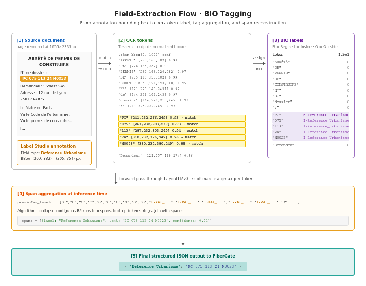
\includegraphics[width=0.85\textwidth,max width=\textwidth]{images/image62.png}
  \caption{\textit{\textbf{Figure 5.7.} Field-extraction flow with BIO tagging: annotation bounding boxes are converted into per-token labels through IoU-based matching and span reconstruction.}}
  \label{fig:image62}
\end{figure}

-- 	\textbf{Stage 1 Reading raw annotations.} Each annotation is exported by Label Studio as a rectangle written in percentage coordinates. These coordinates are converted to pixels using the actual size of the rasterised page. Each record then contains the field type (one of the twelve classes) and the bounding box as the tuple (x\textit{0}, y\textit{0}, x\textit{1}, y\textit{1}).

-- 	\textbf{Stage 2 Parallel OCR view.} Tesseract returns a list of OCR tokens, each with its own pixel-level bounding box and a confidence score. The annotations from Stage 1 and the OCR token boxes from Stage 2 are now in the same pixel reference frame, so they can be compared directly.

-- 	\textbf{Stage 3 Geometric matching.} For each annotation rectangle, the algorithm goes through every OCR token on the page and computes the intersection-over-union (IoU) between the token box and the annotation rectangle. IoU is the ratio of the overlapping area to the total combined area, and takes values between 0 and 1. A token is assigned to the field whenever its IoU is above 0.30, a value chosen on a held-out subset of pages. This threshold is intentionally low, because OCR boxes tend to be smaller than the rectangles drawn by hand, so a stricter threshold would reject too many valid matches. Among the matched tokens, the first one gets the label B-\{field\}, the next contiguous tokens get I-\{field\}, and all other tokens on the page get O.

-- 	\textbf{Stage 4 Subword reconciliation.} The RoBERTa tokeniser used by LayoutLMv3 can split a single OCR word into several sub-tokens. To avoid adding redundant supervision, only the first sub-token of each OCR word receives the BIO label. All continuation sub-tokens, together with the [CLS], [SEP], and padding positions, are assigned the value -100, which tells the cross-entropy loss to ignore them. The final output for each page is a vector of length 512 over 25 label classes plus the -100 mask.

The resulting token-label distribution is shown in Figure 5.8. The O class represents 95.2\% of training tokens, compared to 1.6\% for B- tokens and 3.2\% for I- tokens. This strong skew justifies the use of inverse-frequency weighting at the token level, in the same way it was applied at the document level for the classifier.

\begin{figure}[H]
  \centering
  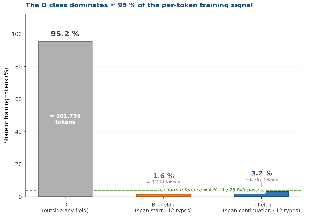
\includegraphics[width=0.85\textwidth,max width=\textwidth]{images/image63.png}
  \caption{\textit{\textbf{Figure 5.8.} Token-label distribution in the extractor training corpus. The O class accounts for 95.2\% of training tokens, against 1.6\% for B- tokens and 3.2\% for I- tokens.}}
  \label{fig:image63}
\end{figure}

\subsection{Warm-Started Extractor Training Protocol}

The extractor is initialised with the trained backbone weights of the classifier. Only the sequence-classification head is replaced by a freshly initialised token-classification head. This warm-start strategy gives the extractor a backbone that has already adapted to the visual style and language of Guichet OI documents. In practice, it reduces the extractor training time by about 40\% compared to starting from the generic LayoutLMv3 checkpoint. The configuration is almost the same as for the classifier (see Table 5.8), with two differences: a slightly smaller maximum number of epochs (fifteen instead of twenty), because the warm start makes convergence faster, and a 25-logit per-token output head instead of the 6-logit document-level head.

\begin{table}[H]
  \centering
  \caption{\textit{\textbf{Table 5.8.} Side-by-side training configuration of the classifier and extractor heads.}}
  \renewcommand{\arraystretch}{1.3}
  \begin{tabularx}{\textwidth}{|X|X|X|}
    \hline
    \textbf{Configuration} & \textbf{Classifier} & \textbf{Extractor} \\ \hline
    Initialisation & layoutlmv3-base & Classifier backbone (warm start) \\ \hline
    Learning rate / schedule & 2 $\times$ 10\textsuperscript{$-$}\textsuperscript{5}, warm-up 10\% + linear decay & Identical \\ \hline
    Training epochs & 20 (patience 5) & 15 (patience 5) \\ \hline
    Effective batch size & 16 (4 $\times$ 4 grad. accum.) & Identical \\ \hline
    Output head & Linear 768 $\rightarrow$ 6 class logits & Linear 768 $\rightarrow$ 25 BIO logits per token \\ \hline
    Loss & Weighted CE on [CLS] & Weighted CE per token, ignore\_index = -100 \\ \hline
    Class weights & Inverse-frequency over 6 classes & Inverse-frequency over 25 BIO classes \\ \hline
    Optimiser / precision & AdamW / FP16 & AdamW / FP16 \\ \hline
    Output at inference & Class + softmax confidence & Per-token BIO, decoded into field spans \\ \hline
    Initialisation & layoutlmv3-base & Classifier backbone (warm start) \\ \hline
    Learning rate / schedule & 2 $\times$ 10\textsuperscript{$-$}\textsuperscript{5}, warm-up 10\% + linear decay & Identical \\ \hline
    Training epochs & 20 (patience 5) & 15 (patience 5) \\ \hline
  \end{tabularx}
\end{table}

\section{Experimental Evaluation and Results}

The evaluation is done on the 133-document held-out test set and works at two levels. Token-level metrics, computed as per-class precision, recall, and F1, are used as a diagnostic, because they show whether the model has at least partly learned the boundaries of each field. Span-level metrics are the main numbers reported in this chapter. A span is counted as a true positive only when both the predicted label and the exact character sequence match the ground truth. This strict rule was chosen because it reflects directly whether the extracted value could be used in the LOC PAR workflow without any human correction.

\subsection{Document Classification Performance Analysis}

The classifier reaches an overall accuracy of 87.7\% on the held-out test set, with a macro-averaged F1 of 0.867. The best validation accuracy observed during training was 89.6\%, and the production checkpoint was chosen on this basis. The per-class breakdown is reported in Table 5.9.

\begin{table}[H]
  \centering
  \caption{\textit{\textbf{Table 5.9.} Document-classifier per-class metrics on the 133-document held-out test set.}}
  \renewcommand{\arraystretch}{1.3}
  \footnotesize
  \begin{tabularx}{\textwidth}{|X|X|X|X|X|}
    \hline
    \textbf{Class} & \textbf{Precision} & \textbf{Recall} & \textbf{F1} & \textbf{Support} \\ \hline
    Authorisation Permit & 0.97 & 0.78 & 0.87 & 37 \\ \hline
    Certificate & 0.92 & 0.73 & 0.81 & 15 \\ \hline
    Information Sheet & 0.98 & 0.98 & 0.98 & 24 \\ \hline
    Mandate & 0.75 & 0.98 & 0.85 & 5 \\ \hline
    Mass Plan & 0.91 & 0.95 & 0.93 & 23 \\ \hline
    Situation Plan & 0.68 & 0.97 & 0.80 & 29 \\ \hline
    Macro Average & 0.87 & 0.90 & 0.87 & 133 \\ \hline
  \end{tabularx}
\end{table}

The Information Sheet class gets the highest F1 (0.98), which can be explained by its very distinctive and consistent visual layout. The Mass Plan class follows with 0.93. The Situation Plan class shows an uneven profile: a high recall (0.97) but a relatively low precision (0.68), which means that the model sometimes labels documents from other categories as Situation Plans. The Mandate class reaches a recall of 0.98 even though it represents only 3.9\% of the training corpus, which confirms that the inverse-frequency weighting from Section 5.2.2 works well. Figure 5.9 shows the per-class F1 distribution and Figure 5.10 shows the training dynamics.

\begin{figure}[H]
  \centering
  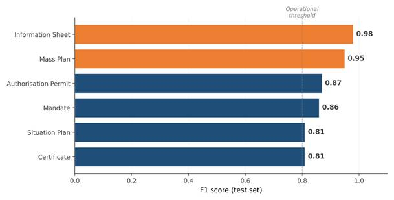
\includegraphics[width=0.85\textwidth,max width=\textwidth]{images/image64.png}
  \caption{\textit{\textbf{Figure 5.9.} Per-class F1 scores on the test set, document classifier.}}
  \label{fig:image64}
\end{figure}

\begin{figure}[H]
  \centering
  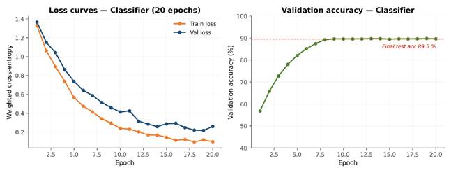
\includegraphics[width=0.85\textwidth,max width=\textwidth]{images/image65.png}
  \caption{\textit{\textbf{Figure 5.10.} Classifier training dynamics}}
  \label{fig:image65}
\end{figure}

\subsection{Field Extraction Performance Analysis}

On the 133-document held-out test set, the best extractor checkpoint (step 301, models/extractor\_v3) reaches a span-level macro-F1 of 0.448 across the twelve fields of the schema. The best F1 observed on the validation set during training was 0.620. Performance varies a lot between fields. Two fields go above F1 = 0.75 and reach the threshold where automated extraction can reasonably replace manual verification. Three fields, on the other hand, stay at F1 = 0.000 and need more annotated examples before they can be used in production. The full per-field results, taken directly from the trainer-state log of the deployed checkpoint, are reported in Table 5.10.

\begin{table}[H]
  \centering
  \caption{\textit{\textbf{Table 5.10.} Per-field span-level metrics on the 133-document held-out test set}}
  \renewcommand{\arraystretch}{1.3}
  \footnotesize
  \begin{tabularx}{\textwidth}{|X|X|X|X|X|X|}
    \hline
    \textbf{Field} & \textbf{Precision} & \textbf{Recall} & \textbf{F1} & \textbf{Train N} & \textbf{Tier} \\ \hline
    Reference\_Urbanisme & 1.000 & 0.862 & 0.926 & 207 & Strong \\ \hline
    Representant\_Nom\_Complet & 0.667 & 1.000 & 0.800 & 18 & Strong \\ \hline
    cabinet\_conseil (Commercial Operator) & 0.667 & 0.800 & 0.727 & 71 & Acceptable \\ \hline
    Representant\_Email & 0.500 & 1.000 & 0.667 & 17 & Acceptable \\ \hline
    DLPI & 1.000 & 0.364 & 0.533 & 71 & Acceptable \\ \hline
    Representant\_Telephone & 0.333 & 1.000 & 0.500 & 17 & Acceptable \\ \hline
    Disposition\_Mandat & 0.308 & 1.000 & 0.471 & 69 & Weak \\ \hline
    nb\_log\_totale & 0.375 & 0.429 & 0.400 & 63 & Weak \\ \hline
    Batiment\_Adresse & 0.233 & 0.714 & 0.351 & 133 & Weak \\ \hline
    Nb\_log\_res & 0.000 & 0.000 & 0.000 & 63 & Critical \\ \hline
    Nb\_log\_pro & 0.000 & 0.000 & 0.000 & 61 & Critical \\ \hline
    Nombre\_Logement\_Lot\_MacroLot & 0.000 & 0.000 & 0.000 & 4 & Critical \\ \hline
    Macro & 0.423 & 0.557 & 0.448 &  &  \\ \hline
  \end{tabularx}
\end{table}

\begin{figure}[H]
  \centering
  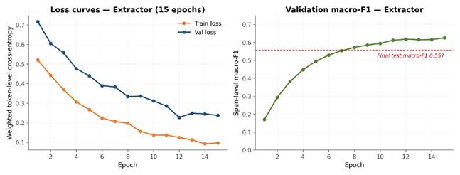
\includegraphics[width=0.85\textwidth,max width=\textwidth]{images/image66.png}
  \caption{\textit{\textbf{Figure 5.11.} Extractor training dynamics}}
  \label{fig:image66}
\end{figure}

A few observations follow from these results. The strongest field by a clear margin is Reference\_Urbanisme (F1 = 0.926). Its consistent PC/PA/DP code pattern, together with its high frequency in the training corpus (207 annotated spans), makes it the most reliable field in the whole schema. The next group of fields contains identity information that follows a clear template: representative full name (0.800), commercial operator name (0.727), and email address (0.667). The weakest fields share one common point: they are numeric values that sit inside dense tables (Nb\_log\_pro, Nb\_log\_res, Nombre\_Logement\_Lot\_MacroLot, all at F1 = 0.000). The visual cues that tell one column from another are written in the column header, which does not always fit together with the target cell inside the 512-token context window of LayoutLMv3. As a result, the model often picks the value from the wrong column. These fields are the main target of the continuous-improvement loop described in Section 5.6.2 .

\subsection{Error Analysis and Confidence-Gated Deployment Strategy}

A close look at the predictions on the test set reveals three failure modes that explain most of the remaining errors:

-- 	\textbf{Header dislocation in housing-count extraction.} When the column header falls outside the 512-token window, the model assigns the value to a neighbouring column. The prediction looks confident but is wrong.

-- 	Span fragmentation in Disposition\_Mandat\textbf{.} LayoutLMv3 treats line breaks as hard boundaries between spans. A disposition that spans two or three lines is therefore cut into several short pieces instead of being read as one full value.

-- 	Spatial ambiguity in Batiment\_Adresse\textbf{.} This field is sometimes predicted as the letterhead address instead of the project address in the body. Both addresses look exactly the same, and only their position on the page tells them apart. When the letterhead is located in a region that looks similar to the project-address region, the model cannot decide reliably.

To turn this uneven performance into a controlled behaviour in production, a confidence-based routing policy is applied at inference time. For fields whose test-set F1 is 0.70 or above, predictions are sent directly to the workflow if the mean per-token softmax confidence is above 0.60; otherwise they are shown to the consultant as a draft to review. For fields whose test-set F1 is below 0.70, every prediction is routed to manual verification, regardless of the confidence value. The effect of this policy is to turn the bimodal performance profile into a smooth degradation at the application level: the strongest fields are fully automated, the middle ones are pre-filled and reviewed, and the weakest ones stay under human control until the lifecycle activities of Section 5.6.2 raise them above the threshold.

\section{Service Lifecycle Management}

\subsection{Production Inference Workflow and Rule-Based Post-Processing}

At inference time, an incoming document (PDF or PNG/JPG) is processed by the same preprocessing chain that produced the training data. This guarantees that the system behaves consistently between training and deployment. PDF files are rasterised with pdf2image at a target resolution of about 1,655 $\times$ 2,335 pixels. OCR is then run with Tesseract 5 and a French language model. The output of this stage is a JSON object containing four parallel arrays: the tokenised words, their pixel-level bounding boxes, the same bounding boxes normalised to the [0, 1000] range expected by LayoutLMv3, and the per-token confidence scores. This four-array structure is the standard interface between the OCR layer and the LayoutLMv3 model.

The preprocessed page is then passed through the two models: the classifier predicts the document class, and the extractor produces a JSON dictionary that maps each field name to its extracted value. This JSON payload is the only output of the trained neural models. Two rule-based Python modules, neither of which contains any learned parameters, read this payload downstream:

-- 	\textbf{Completeness recommendation engine:} applies the LOC PAR business rules and produces a completeness verdict for each demand.

-- 	\textbf{CMS pre-fill generator:} writes a 27-column Excel file that follows the operational template. Any field that could not be extracted with enough confidence is flagged for manual completion, using information from the internal Optimum platform of Orange.

Both modules were kept from the proof of concept without changes. The correctness of the CMS pre-fill generator depends entirely on the mapping table between extracted field names and CMS column indices, which is checked through dedicated unit tests. To make qualitative inspection easier, a small Streamlit front-end was built. Figures 5.12 and 5.13 show the interface for a complete and an incomplete demand, and Figure 5.14 shows the resulting CMS file.

\begin{figure}[H]
  \centering
  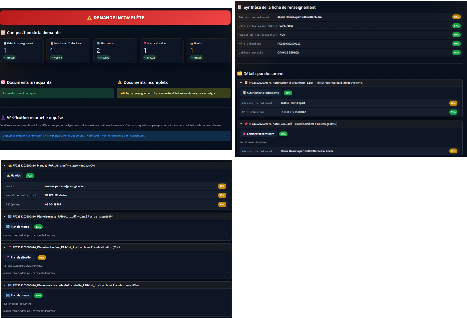
\includegraphics[width=0.85\textwidth,max width=\textwidth]{images/image67.png}
  \caption{\textit{\textbf{Figure 5.13.} Inference output for an incomplete demand (DEMANDE INCOMPLETE)}}
  \label{fig:image67}
\end{figure}

\begin{figure}[H]
  \centering
  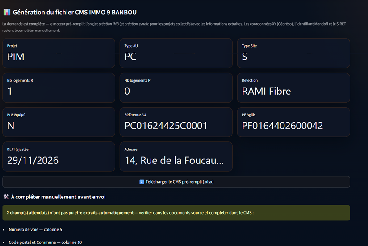
\includegraphics[width=0.85\textwidth,max width=\textwidth]{images/image68.png}
  \caption{![][image69]}
  \label{fig:image68}
\end{figure}

\subsection{Model Versioning and Continuous Improvement Framework}

The continuous-improvement framework runs three coordinated activities in parallel with daily inference, as shown in Figure 5.15:

-- 	\textbf{Correction capture.} Every correction made by a consultant on an AI-extracted field through the unified web platform is saved as a candidate annotation for the next training pass. Each correction is paired with the original OCR tokens, the page coordinates, and a reference to the source document, so that no supervision signal is lost between the correction and the next fine-tuning step.

-- 	\textbf{Versioned checkpoints.} Each training pass produces a versioned checkpoint, stored under the naming convention models/classifier\_v\{n\} and models/extractor\_v\{n\}. A candidate checkpoint is promoted to production only if it beats the currently deployed model on macro-F1 on both heads. This rule ensures that the production system never regresses in aggregate performance.

-- 	\textbf{Inference auditability.} The inference service exposes the active model version through its /health endpoint. This allows the web platform to link every prediction to a specific checkpoint and to monitor performance drift over time. Together with correction capture, this closes the loop between the production system and the training corpus.

\begin{figure}[H]
  \centering
  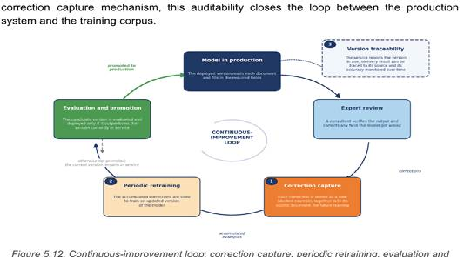
\includegraphics[width=0.85\textwidth,max width=\textwidth]{images/image70.png}
  \caption{\textit{\textbf{Figure 5.15.} Continuous-improvement loop: correction capture, periodic retraining, evaluation and promotion, and inference auditability run in parallel with daily production inference.}}
  \label{fig:image70}
\end{figure}

\section*{Conclusion}
\addcontentsline{toc}{section}{Conclusion}

This chapter has described the full engineering trajectory of the FiberGate AI Service. Starting from the limitations of the proof of concept, the per-type hybrid pipeline was replaced by a unified multimodal architecture based on LayoutLMv3, which was chosen through a systematic comparison of six candidate models. A corpus of 872 annotated documents was built with Label Studio, and the class imbalance was handled through inverse-frequency weighting in the CrossEntropyLoss function during the training of both the classifier and the extractor. The source-PDF-level split adopted in Section 5.2.2 prevents the data leakage that a page-level split would have caused, so all the evaluation figures in this chapter rest on a clean partition.

The document classifier reaches 87.7\% accuracy and a macro-F1 of 0.867 on the 133-document held-out test set. The field extractor reaches a span-level macro-F1 of 0.448 across the twelve fields of the schema: two fields go above F1 = 0.75 and qualify for full automation, four occupy an acceptable middle range suitable for review-assisted deployment, and three need more annotated examples before production use. The confidence-gated policy of Section 5.5.3 turns this uneven performance into a controlled deployment posture, keeping automation on the reliable fields while sending uncertain predictions to manual verification. Finally, the lifecycle framework of Section 5.6.2 ensures that every consultant correction is captured and folded back into periodic retraining cycles, giving the weaker fields a clear path to reach the operational threshold over time. The next chapter turns to the third pillar of the project: the unified web platform that brings the FiberGate AI Service and the SENTINEL fleet together into a single operational tool.
